\documentclass[10pt]{article}
\usepackage[margin=0.9in]{geometry}
\usepackage{amsmath,amssymb}
\usepackage{booktabs}
\usepackage{enumitem}
\usepackage{graphicx}
\usepackage[T1]{fontenc}
\usepackage[hidelinks]{hyperref}
\usepackage{caption}
\captionsetup{font=small,labelfont=bf,skip=3pt}
\setlist{nosep,leftmargin=1.3em}
\setlist[description]{style=unboxed,leftmargin=1.3em,labelindent=0pt,itemsep=1pt}
\graphicspath{{../results/}}
\setlength{\parskip}{2pt}
\newcommand{\Fanon}{\mathcal{F}^{\mathrm{anon}}}
\newcommand{\Fid}{\mathcal{F}^{\mathrm{id}}}
\newcommand{\For}{\mathcal{F}^{\mathrm{oracle}}}

\title{\vspace{-1.2em}\textbf{Rent or Toxicity? Strategic Exploitability of Learning Market Makers\\ with Public Wallet Information}\\[0.2em]\large Workshop 1 report}
\author{Deepu Pradeep \quad Miguel Betran Menz\\
\normalsize 6.S974 Games, Learning, and Security --- Example 4 (Algorithmic Market with Adaptive Agents)}
\date{October 27, 2026}

\begin{document}
\maketitle
\vspace{-1.5em}

\section{Problem and contributions}
Independent learning agents that post prices settle on payoffs above the competitive level without communicating. Is that payoff \emph{rent} an adversary can take, or the correct price of trading against a better-informed opponent? The two look identical from outside, and we study the difference on Hyperliquid, an on-chain market in which every trade carries the public identity of both parties, so that what an adversary is allowed to know is a design choice of the venue. The game has four roles: a \emph{venue} that sets the rules, \emph{incumbents} (the defenders) that learn to post prices, \emph{takers} (nature, with a hidden state) that accept or decline them, and an \emph{entrant} (the adversary) that best-responds with a chosen information set. Three questions: what information is worth to the adversary (RQ1); whether the defenders' rent makes them more exploitable (RQ2); and which defences, the makers' own and the venue's, hold up (RQ3). Since the October 6 proposal:
\begin{enumerate}
\item Learning defenders coordinate above the competitive point in every configuration tried (rent index $0.71$--$0.87$, ten seeds), by restraint, not by failing to explore (\S\ref{sec:r1}).
\item Rent is exploitable in proportion to its size, not more: a profit-maximising adversary destroys a fraction $\approx0.7$ of it whatever the rent, with at most a weak dependence on it, across 180 defender populations (\S\ref{sec:r2}). The hypothesis of the proposal holds only in its trivial form.
\item Identity pays not because wallets repeat (they almost never do) but because informed flow clusters in time and a wallet's trade reveals the hidden state before the price does; its value grows with the delay before outcomes become public, up to the lifetime of the state (\S\ref{sec:r3}).
\item On Hyperliquid the quoted spread on the major books is one tick essentially always, so rent cannot live in the price; the average fill at the best price loses within ten seconds; and the ten most active makers break even or earn at the same price where everyone else loses, persistently across days (\S\ref{sec:r4}).
\item In the game where the price cannot move, identity is worth more against defenders that learn to select, not less, and the identity-blind resting liquidity absorbs the informed flow (\S\ref{sec:r5}).
\end{enumerate}
Code, results and a running findings log: \url{https://github.com/pradeepu191/wargame}.

\section{Definitions and notation}\label{sec:defs}
Every market term used below is defined here once, in the language of games and control, and then used freely.
\begin{description}
\item[Quote, half-spread $h$ (the action); tick $\theta$.] A maker's standing offer to sell at $m_t+h\theta$ and buy at $m_t-h\theta$ around the public reference price $m_t$ (the \emph{mid}), $h\in\{1,\dots,K\}$; $\theta$ is the grid of the action space. The \emph{best quote} or \emph{touch} is the lowest $h$ among makers; the taker always hits it.
\item[Fundamental $V_t$; informed and uninformed takers; adverse selection.] $V_t=m_t\pm d$, $d\sim\mathrm{Exp}(\mu)$, is the state. With probability $\alpha$ the taker knows it and accepts only when the maker loses, costing the maker exactly $\mu$ in expectation at every $h$; otherwise she trades for private reasons unrelated to the state. \emph{Adverse selection} is the expected loss from being matched with the informed type; \emph{toxic} flow has a high informed share.
\item[Payoff function, Nash point, monopoly point.] $\Pi(h;\alpha)=(1-\alpha)\,2x\bar\Phi(x/\sigma_L)-\alpha\mu e^{-x/\mu}$, $x=h\theta$, is a maker's expected one-period payoff when it holds the best quote. $h^C$, the smallest $h$ with $\Pi\ge0$, is the Nash equilibrium of the one-shot pricing game (at any $h>h^C$ a maker gains by moving to $h-1$: \emph{undercutting}); $h^M=\arg\max\Pi$ is the joint-monopoly action; $\Pi^C,\Pi^M$ the payoffs there.
\item[Rent index $\Delta$, $C(\pi)$.] $(\bar\Pi-\Pi^C)/(\Pi^M-\Pi^C)\in[0,1]$: where a population sits between Nash (0) and joint monopoly (1); $\Delta$ while learning, $C(\pi)$ for a frozen policy profile. A profile with $C>0$ sustained by independent learners that never communicate is \emph{tacit collusion}. \emph{Restraint}: forgoing the undercut in states where it is the myopic best response.
\item[Exploitability.] $\Pi_{\mathrm{nominal}}(\pi)$ is the frozen defenders' payoff alone; $J(\pi;A)$ with adversary $A$; $L^A_{\mathrm{BR}}=\Pi_{\mathrm{nominal}}-J$ the defenders' loss (the game is general-sum, so the defenders' loss, not the adversary's gain, is the statistic); $\kappa_A=L^A_{\mathrm{BR}}/(\Pi_{\mathrm{nominal}}-\Pi^C)$ the fraction of rent destroyed. \emph{Rent units}: payoffs divided by $\Pi^M-\Pi^C$.
\item[Information sets.] $\Fanon$ (public tape and book) $\subset\Fid$ (plus the wallet on every print) $\subset\For$ (plus the hidden state). \emph{Value of identity}: $\pi^{\mathrm{id}}-\pi^{\mathrm{anon}}$, read from the venue's side as the price of anonymity.
\item[Wallet types, regime, mark lag.] Wallet $j$ is informed with probability $\alpha_j$ (stratified $\mathrm{Beta}$ quantiles, mean $\bar\alpha$, concentration $\kappa_\alpha$). A hidden Markov state $z_t\in\{\text{calm},\text{toxic}\}$ with persistence $\rho_z$ governs which wallets are active. A print's realized payoff (its \emph{mark}) becomes public $L$ arrivals later. From the entrant's side this is a POMDP; its policy carries a belief over $z_t$ and acts on $\alpha_{\mathrm{next}}$, the implied probability that the next taker is informed.
\item[Queue game.] The same environment with the spread fixed at one tick: the action is \emph{rest} (keep a standing offer at the touch) or \emph{out}; makers at the same price are served first-in-first-out (\emph{time priority}), and a maker that withdraws rejoins at the back. Expected payoff of a fill at $h$ against type $\alpha$: $(1-q)x-q\mu$, $q$ the probability the fill was informed. \emph{Selection} is choosing which fills to take.
\item[On data.] \emph{Markout at $\tau$}: a maker's ex-post payoff on one fill against the mid $\tau$ seconds later, in basis points ($10^{-4}$) of the price; it includes the half-spread earned. \emph{Effective spread}: what the taker paid relative to the last mid before the fill. A fill \emph{at the touch} printed at the best quote of that book; a \emph{walked} fill printed beyond it (the order swept several prices).
\end{description}

\section{Model}
One contract, discrete periods, $N$ makers on a tick grid ($\theta=0.5$, $K=24$, $\sigma_L=8$, $\mu=5$), one taker per period, $T=100$ periods per episode. Benchmarks are closed-form: $(h^C,h^M)=(2,13),(4,14),(8,17)$ and $\Pi^M-\Pi^C=1.90,1.38,0.66$ at $\bar\alpha=0.1,0.3,0.5$: less rent is available where flow is more toxic. Takers are drawn from $M=50$ wallets with types $\alpha_j$, under the regime $z_t$ (at $\kappa_\alpha=1$ the two states have toxicity $0.15$ and $0.65$ around $\bar\alpha=0.3$) and the mark lag $L$. Incumbents are tabular Q-learners (state: own and best rival's last quote) trained for $12{,}000$ episodes and then frozen; the entrant observes one of $\Fanon,\Fid,\For$, runs an exact Bayesian filter over the regime, and quotes the break-even for $\alpha_{\mathrm{next}}$, undercutting the incumbents when that leaves at least one tick. Two modes of the same environment: the spread free (above), or pinned at one tick (the queue game, \S\ref{sec:r5}). Every number is a mean over independently trained seeds with a 95\% interval; comparisons between information sets are paired within a seed under common random numbers. Data: 327 hours of signed trades on BTC, ETH, SOL and HYPE from the public feed (October 7--20, 2026), fifteen hours of top-of-book at every change in two sessions eight days apart, and the January 2026 archive of \cite{albers} for the archive-vs-feed check.

\section{Results}
\subsection{Learners coordinate above the Nash point}\label{sec:r1}
Two or three Q-learners settle at half-spreads of $10.6$, $14.4$, $17.4$ ticks at $\bar\alpha=0.1,0.3,0.5$ against Nash $2,4,8$ and monopoly $13,14,17$: $\Delta=0.83,0.86,0.77$ (seed sd $0.01$--$0.02$), replicating \cite{cfl}. A grid at $\bar\alpha=0.3$ over $N\in\{2,3,5\}$, learning rate $\in\{0.05,0.15\}$ and initialisation gives $\Delta=0.71$--$0.87$ in every cell (Table~\ref{tab:robust}). The mechanism test says this is restraint: in 55--83\% of visited states a rival sits at or inside the monopoly quote, and in 96--100\% of those the learner's greedy action forgoes the undercut. The best quoter changes between episodes 45--70\% of the time: turn-taking, not a leader.

\begin{table}[h]\footnotesize\centering
\begin{tabular}{cccccc}
\toprule
$N$ & learning rate & half-spread & $\Delta$ & restraint $\mid$ contested & leader switch \\
\midrule
2 & 0.05 / 0.15 & 11.2 / 14.4 & 0.84 / 0.86 & 1.00 / 0.99 & 0.52 / 0.45 \\
3 & 0.05 / 0.15 & 9.3 / 14.9 & 0.72 / 0.86 & 0.98 / 0.99 & 0.61 / 0.58 \\
5 & 0.05 / 0.15 & 9.7 / 15.0 & 0.71 / 0.87 & 0.97 / 0.99 & 0.63 / 0.62 \\
\bottomrule
\end{tabular}
\caption{Robustness grid at $\bar\alpha=0.3$, ten seeds; $h^C=4$, $h^M=14$.}\label{tab:robust}
\end{table}

\subsection{Rent is exploitable in proportion, not more (RQ2)}\label{sec:r2}
180 frozen populations ($C$ from $0.42$ to $0.97$) each face four adversaries for 500 episodes: the competitive quoter (quotes $h^C$), the one-tick undercutter, the \emph{markout} entrant (best-responds from its own fills' realized payoffs) and the \emph{oracle} (the same rule handed the true $\bar\alpha$). Figure~\ref{fig:exploit}. The literal hypothesis $\partial L_{\mathrm{BR}}/\partial C>0$ holds by construction: the adversary that hurts the defenders most is the competitive quoter in 179 of 180 populations, it pushes them below $\Pi^C$, so $L_{\mathrm{BR}}\approx\Pi_{\mathrm{nominal}}$ and the slope is one ($1.03\ [1.00,1.07]$ at $\bar\alpha=0.3$). The substantive version is not supported: $\kappa_A$, the fraction a profit-maximising adversary destroys, is $0.71$--$0.73$ for the undercutter, the markout and the oracle entrant across the whole range of $C$; pooled and within-cell slopes include zero, and at $\bar\alpha=0.3$ the slope is $+0.23$ to $+0.25$ with intervals just excluding zero but no significant rank correlation---at most $0.13$ in $\kappa_A$ over the observed range. Damage and profit are different objectives: the competitive quoter earns $0.10$ rent units, the profit-maximisers $0.48$--$0.51$ and leave the defenders 27--30\% of their rent. Knowing the true $\bar\alpha$ adds nothing over estimating it from own fills ($0.49$ vs $0.51$): in a stationary market the tape carries the full value of the toxicity \emph{level}---which is what sent us to a non-stationary one.

\begin{figure}[h]\centering
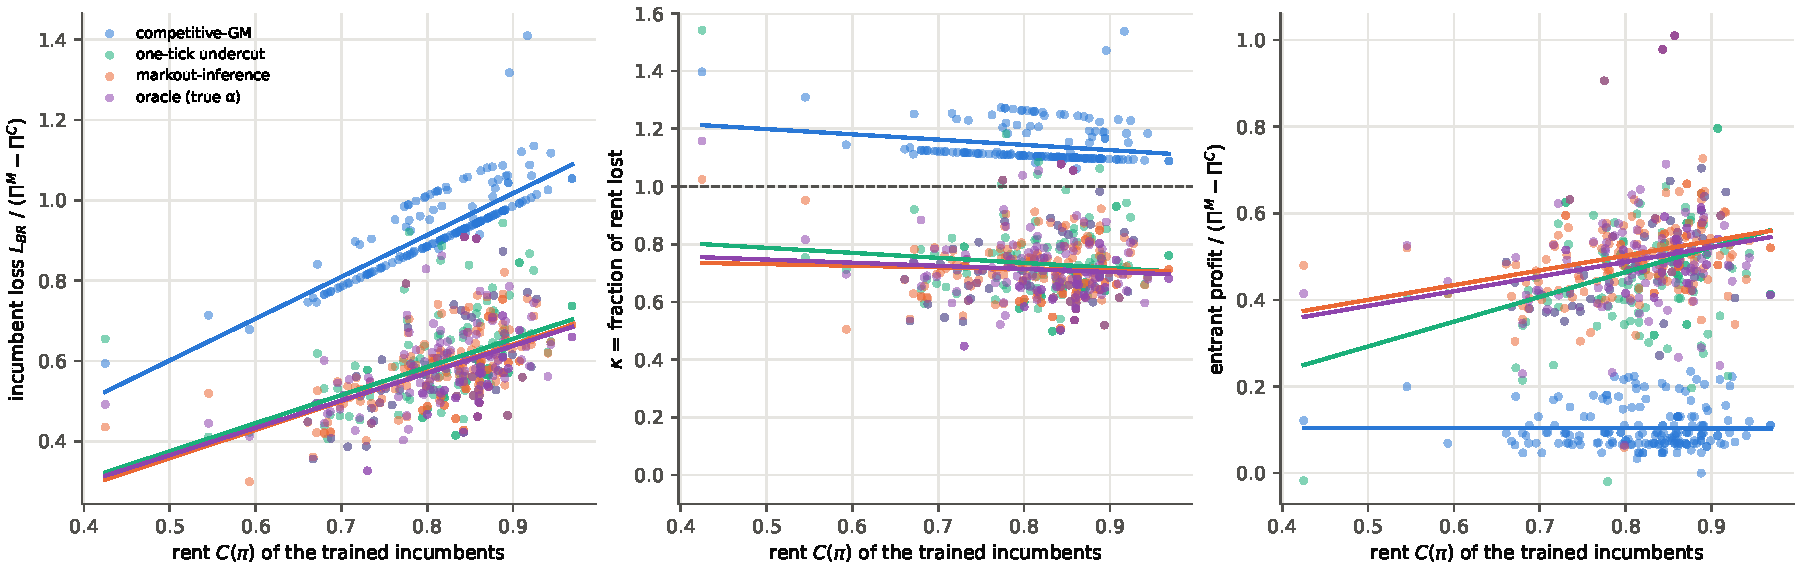
\includegraphics[width=0.92\textwidth]{fig_exploitability_10seed.pdf}
\caption{Defenders' loss, fraction of rent destroyed, and adversary payoff against the defenders' rent $C(\pi)$; 180 populations, one point per population and adversary.}\label{fig:exploit}
\end{figure}

\subsection{What identity is worth, and why (RQ1)}\label{sec:r3}
The proposal's mechanism---wallet toxicity is a persistent trait, so the last wallet predicts the next---is worth $+0.15$ to $+0.30$ rent units in the simulator when wallets repeat ($\rho=0.9$--$0.99$, ten of ten seeds) and exactly zero when they do not. On Hyperliquid they do not: the same-wallet repeat rate at the order level is $0.02$--$0.05$. Yet identity predicts the next fill's toxicity there: conditioning on whether the previous taker was a toxic wallet moves the next fill's markout by $0.5$--$1.0$ bps, and 78--99\% of that survives conditioning on what an anonymous quoter sees (whether the price has already moved against the previous maker, which by the next arrival it has only one time in five). The mechanism the data support is the regime plus the lag: informed flow clusters in time, and a toxic wallet's print reveals the state before the price does. With that in the simulator identity's value reappears where it should (Figure~\ref{fig:lag}): at $\bar\alpha=0.5$ it grows with the mark lag from $+0.06$ to $+0.16$ rent units ($\pm0.07$) at $\rho_z=0.99$, and from $+0.06$ to a peak of $+0.11$ at $L=20$ when $\rho_z=0.9$---the peak is the regime's lifetime, beyond which the tape was useless anyway. \emph{Identity's value grows with the delay before outcomes are public, up to the lifetime of the state.} It is small ($+0.02$ to $+0.04$) at $\bar\alpha=0.3$ and zero at $\bar\alpha=0.1$: against a cartel quoting far above break-even even the toxic state leaves an undercut profitable, so the state is not decision-relevant---a prediction about \emph{which} books reward identity. One tail is worth recording: when types are close together ($\kappa_\alpha=5$) and identity carries little, three of ten cartels punish the better-informed entrant, whose moving quote triggers their learned reaction while the anonymous entrant's steady undercut does not. Information used naively can provoke the defenders; the reaction function is part of the game.

\begin{figure}[h]\centering
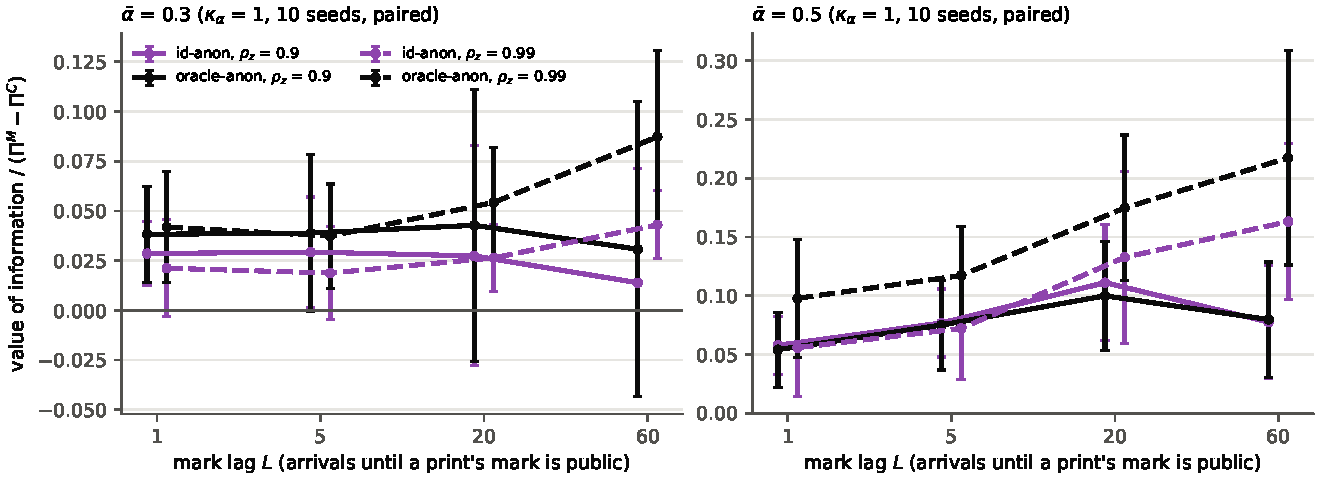
\includegraphics[width=0.9\textwidth]{fig_cfl_exp2_marklag_10seed.pdf}
\caption{Value of identity (id $-$ anon) and of the true state (oracle $-$ anon) in rent units against the mark lag $L$; paired per seed, ten seeds, 95\% intervals, $\kappa_\alpha=1$.}\label{fig:lag}
\end{figure}

\subsection{Hyperliquid: the price cannot move, and someone still earns the spread}\label{sec:r4}
Table~\ref{tab:data}. The quoted spread on BTC, ETH and SOL is one tick essentially all the time (the 90th percentile equals the median), so on those books a rent cannot appear as a wider quote. A fill at the touch pays exactly that tick---the check that the book is aligned to the trade---and then loses $0.3$--$0.6$ bps to the mid within ten seconds on every coin; the taker's cost is in depth, not the quote: one order in ten walks the book and pays twenty ticks, and on the deep books those are the informed ones (walked fills lose $-0.8$ / $-2.3$ bps on BTC/ETH, earn on HYPE/SOL). Every print carries the maker's wallet, so the RQ3 anchor can be read directly (Figure~\ref{fig:makers}): the ten most active market-maker wallets (chosen on activity over the full window, not on the outcome) break even or earn at ten seconds where the other market makers and, most of all, the makers that are not market makers lose; at the \emph{same price}, fills at the touch, they earn $0.4$--$1.1$ bps per fill more than everyone else, and their ranking persists across two recording nights eight days apart (rank correlation $0.43$--$0.75$, $p<10^{-3}$). Makers playing the same action get different fills; the difference is when they are at the front of the line. Makers who select earn the spread; identity-blind resting liquidity is the counterparty.

\begin{table}[h]\footnotesize\centering
\resizebox{\linewidth}{!}{%
\begin{tabular}{lcccc}
\toprule
 & BTC & ETH & HYPE & SOL \\
\midrule
quoted spread, median (bps); one tick & 0.12; 0.12 & 0.42; 0.39 & 0.13; 0.11 & 0.96; 0.86 \\
effective spread: fills at the touch / walked / per order & 0.13 / 2.35 / 0.27 & 0.43 / 3.20 / 0.60 & 0.18 / 3.57 / 0.40 & 0.95 / 5.20 / 1.09 \\
10-s markout, all fills; at the touch; walked (bps) & $-0.45$; $-0.37$; $-0.64$ & $-0.61$; $-0.46$; $-1.26$ & $-0.20$; $-0.41$; $+0.04$ & $-0.08$; $-0.26$; $+0.70$ \\
identity given the anonymous signal, next fill (bps, 327 h) & $-0.64$ & $-1.01$ & $-0.59$ & $-0.59$ \\
10-s markout: top-10 MM / other MM / non-MM makers & $-0.10$ / $-0.36$ / $-0.88$ & $+0.19$ / $-0.53$ / $-1.25$ & $+0.11$ / $-0.12$ / $-0.71$ & $+0.52$ / $-0.17$ / $-0.41$ \\
at the touch: top-10 / everyone else & $-0.02$ / $-0.41$ & $+0.24$ / $-0.70$ & $+0.09$ / $-0.56$ & $+0.52$ / $-0.56$ \\
rank correlation of per-maker markout, night vs night ($n$) & 0.75 (108) & 0.50 (65) & 0.43 (68) & 0.56 (45) \\
\bottomrule
\end{tabular}}
\caption{Hyperliquid, October 2026: two top-of-book sessions eight days apart (15 hours; 112k / 55k / 106k / 29k marked fills) and 327 hours of signed trades. The walked-fill and per-order effective spreads are from the first session. SEs cluster by five-minute block; all top-10 vs rest gaps exceed four SEs; all rank correlations $p<10^{-3}$.}\label{tab:data}
\end{table}

\begin{figure}[h]\centering
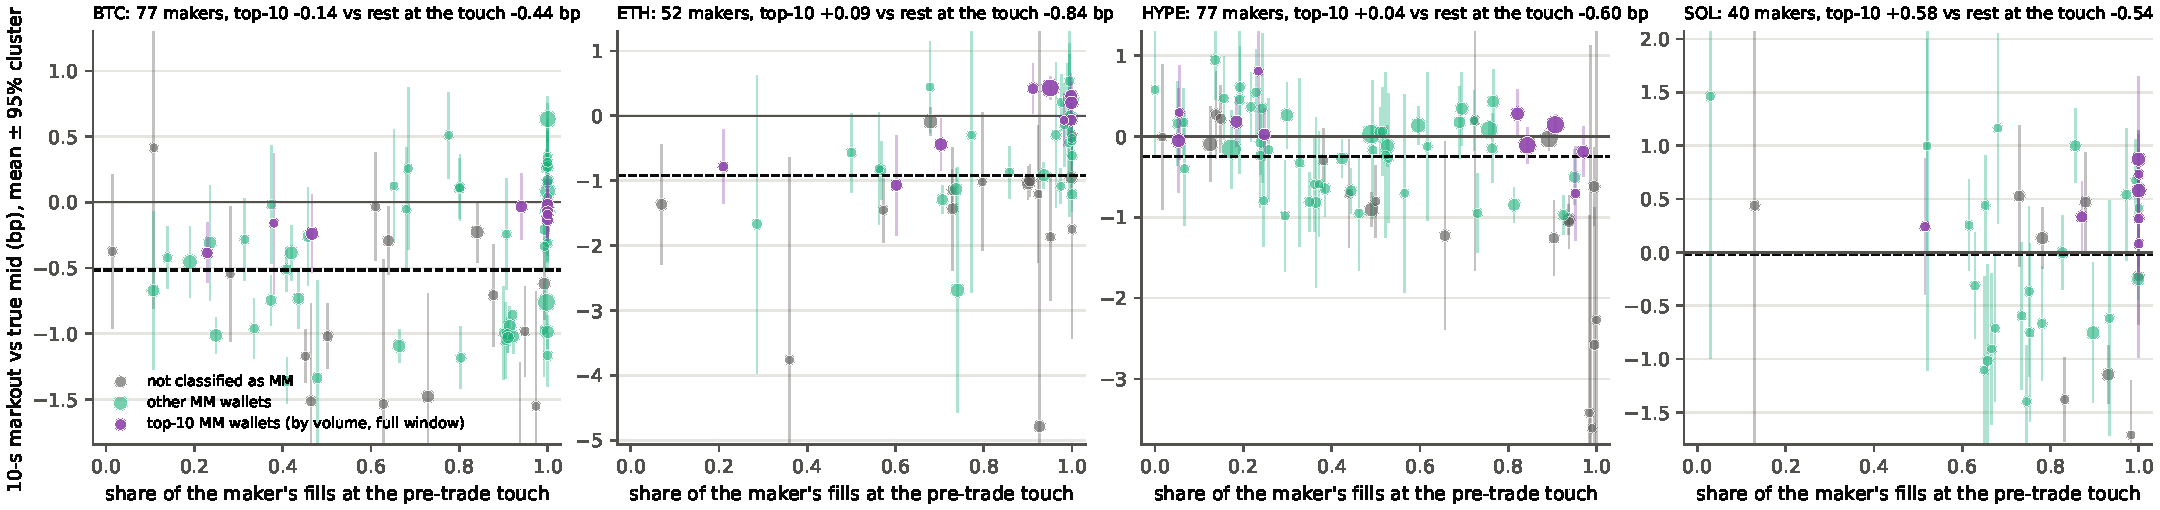
\includegraphics[width=\textwidth]{fig_makers_live_2026_10.pdf}
\caption{Per-maker 10-s markout (bps, mean $\pm$ 95\% cluster interval) against the share of the maker's fills at the touch; one dot per maker with $\ge100$ marked fills over the two sessions; dashed line: all fills.}\label{fig:makers}
\end{figure}

\subsection{The queue game: identity when the price cannot move (RQ3, tick lever)}\label{sec:r5}
With the spread pinned at $h^C$ a fill is worth $+0.15$ on average, $+1.10$ in the calm state and $-2.26$ in the toxic one: all the value is in selection. The population is two incumbents, a \emph{fringe} of two always-resting makers (the retail orders and the vault that never step out; without them two learners that both step out in a toxic spell leave an empty book and a self-fulfilling lock in which nobody rests), and one entrant. Two incumbent types: always-resting (the competitive one-tick book) and \emph{no-regret} learners (EXP3 over the complete policies $\{$always rest, never rest, select on the tape$\}$)---tabular Q-learners cannot learn to queue, because with time priority the reward of resting arrives only after several consecutive periods in line and an $\epsilon$-greedy learner breaks the chain, never reaches the front and flickers. Figure~\ref{fig:queue}. What the incumbents learn: with a fresh tape both become selectors; with a stale one ($L\ge20$ at $\rho_z=0.9$) a third of the weight moves to always-rest; nobody learns to stay out. What identity is worth: $+0.05$ to $+0.06$ per period against incumbents that select, at every lag, five of five seeds, against $+0.03$ to $+0.04$ when they do not---\emph{more} against sophisticated defenders, because once they read the tape an entrant that reads only the tape is one more of them and the wallet tag is what is left; at $\rho_z=0.99$ the increment grows with the lag from $0.00$ to $+0.06$, the same mechanism as \S\ref{sec:r3}. Who pays: the fringe's payoff goes from $+0.00$--$0.03$ with an always-resting entrant to $-0.02$--$-0.04$ with a selecting one ($-0.10$ at $\rho_z=0.99$). The spread game and the queue game give the same answer through different actions: a quoter who knows who just printed takes the benign flow and leaves the toxic flow to identity-blind rivals---by undercutting selectively where undercutting is possible, by resting selectively where it is not---and in the simulator as on Hyperliquid, the always-resting liquidity is the counterparty.

\begin{figure}[h]\centering
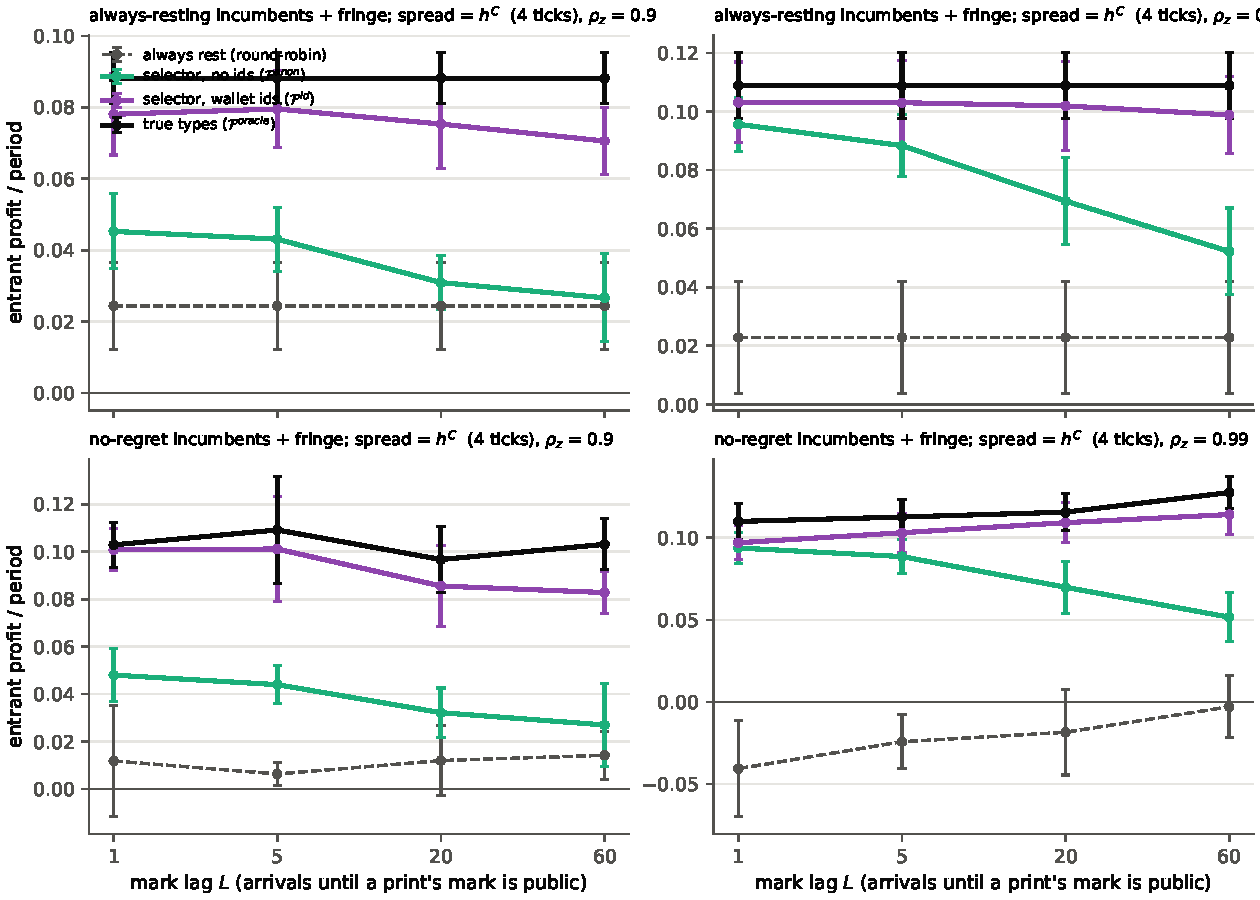
\includegraphics[width=0.95\textwidth]{fig_queue_incumbents.pdf}
\caption{Queue game at break-even: entrant payoff per period by information set against the mark lag, against always-resting (top) and no-regret (bottom) incumbents; $\rho_z=0.9$ (left), $0.99$ (right); five seeds, 95\% intervals.}\label{fig:queue}
\end{figure}

\section{Plan to the November meeting}
\emph{Defences (RQ3), in the same environment.} The venue's priority fee as the price of a place in line; identity-aware incumbents (an identity expert in the no-regret set); the makers' own levers---randomisation, hysteresis, identity-aware control---each reported as a point on the profit--resilience frontier $(\mathbb{E}[\Pi_{\mathrm{nominal}}],\,-\mathrm{CVaR}_{0.05}(\Pi_{\mathrm{attack}}))$ against the three adversaries. \emph{Data.} A multi-day book window from an always-on recorder (intervals on the touch-fill loss and the per-maker persistence by coin and hour); the October 2025 cascade as the stress case; order-level lifecycles (December 2025 archive) to say \emph{how} the top makers select---position, cancellation, depth. \emph{Rigour.} Train at $\bar\alpha$, test at $\bar\alpha'$; held-out adversaries; chronological splits on data. Then a short results note and the discussion of how to organise a submission.

\paragraph{Two questions.} (1) We run the free-spread and the pinned-spread games as two modes of one environment; which should carry the paper, the one with closed-form benchmarks or the one the data say is binding? (2) Of the venue's levers---anonymity, tick, priority fee---which is the security-relevant one from your side?

\begin{thebibliography}{9}\footnotesize
\bibitem{cfl} J.-E. Colliard, T. Foucault, S. Lovo. Algorithmic Pricing and Liquidity in Securities Markets. \emph{Review of Financial Studies}, 2026.
\bibitem{calvano} E. Calvano, G. Calzolari, V. Denicol\`o, S. Pastorello. Artificial Intelligence, Algorithmic Pricing, and Collusion. \emph{AER} 110(10), 2020.
\bibitem{zhai} D. Zhai. Public Trader Identity: Adverse Selection and Return Predictability. arXiv:2608.04373, 2026.
\bibitem{ccp} \'A. Cartea, P. Chang, J. Penalva. Algorithms and Supracompetitive Prices in Electronic Markets: The Impact of Tick Size. SSRN 4105954, 2026.
\bibitem{dgj} W. W. Dou, I. Goldstein, Y. Ji. AI-Powered Trading, Algorithmic Collusion, and Price Efficiency. NBER WP 34054, 2025.
\bibitem{dss} Y. Deng, J. Schneider, B. Sivan. Strategizing against No-Regret Learners. \emph{NeurIPS} 2019.
\bibitem{albers} J. Albers, M. Cucuringu, S. Howison, A. Y. Shestopaloff. An Open Book: Level 4 Order Book Data from the Hyperliquid Exchange. SSRN 6465720, 2026.
\bibitem{hldocs} Hyperliquid Documentation. \url{https://hyperliquid.gitbook.io/hyperliquid-docs}, accessed Oct.\ 2026.
\end{thebibliography}
\end{document}
